%\documentclass{article}
\documentclass{standalone}
\standaloneconfig{border=2mm 2mm 2mm 2mm}
%\usepackage{geometry}
\usepackage{pgfplots}
\pgfplotsset{width=15cm, height=5cm,compat=1.9}
%\pgfplotsset{compat=1.9}

% We will externalize the figures
%\usepgfplotslibrary{external}
%\tikzexternalize

\begin{document}
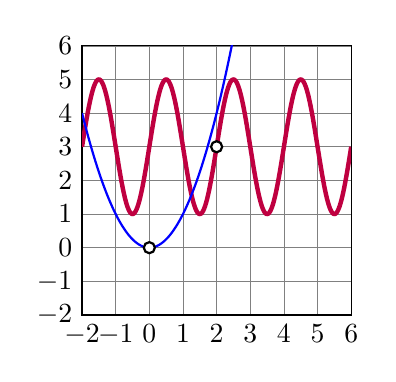
\begin{tikzpicture}
\begin{axis}[
  %axis lines = left,
  width=5cm,
  height=5cm,
  %xlabel ={$x$}, 
  %ylabel = {$y$},
  xmin=-2.0, xmax=6.0,
  ymin=-2.0, ymax=6.0,
  xtick={-2.0,...,6.0},
  ytick={-2.0,...,6.0},
  xmajorgrids=true, ymajorgrids=true,
  minor grid style = {very thin, gray},
  major grid style={solid, very thin, gray},
  xminorgrids=false, yminorgrids=false, minor tick num = 1,
  %grid style = dashed,
  minor x tick num = 9,
  minor y tick num = 4,
  %minor tick style = {thin, gray},
  %major tick style = {thick, black},
  minor tick style={draw=none},
  xticklabel style={/pgf/number format/.cd, fixed relative, precision=4, /tikz/.cd},
  yticklabel style={/pgf/number format/.cd,fixed relative,precision=3}]
  %style="yticklabel style={
  %/pgf/number format/precision=5,
  %/pgf/number format/fixed}",
  %scaled y ticks=false]

%\addplot[color=red]{exp(x)};
%\addplot[color=blue, samples=100]{x^2};ı

\addplot[color=purple, domain=-2.0:6.0, samples=1000, style=ultra thick]{3+2*(sin(deg(x*pi)))};
\addplot[color=blue, domain=-2.0:6.0, samples=1000, style=thick]{x^2};
\addplot[color=black,mark=*,style=thick,fill=white,only marks] coordinates {(0,0) (2,3)};

\end{axis}
\end{tikzpicture}
\end{document}